\chapter{Initial Requirements}

\section{Introduction}
In this project we will create a SDN controller for defense against DDoS attacks. Through a REST API system, a web server can notify the begin of a DDoS attack; the controller will create an address change mechanism from D to D’.

\section{Implementation}
In this project we will implement:

\begin{figure}[H]
\begin{center}
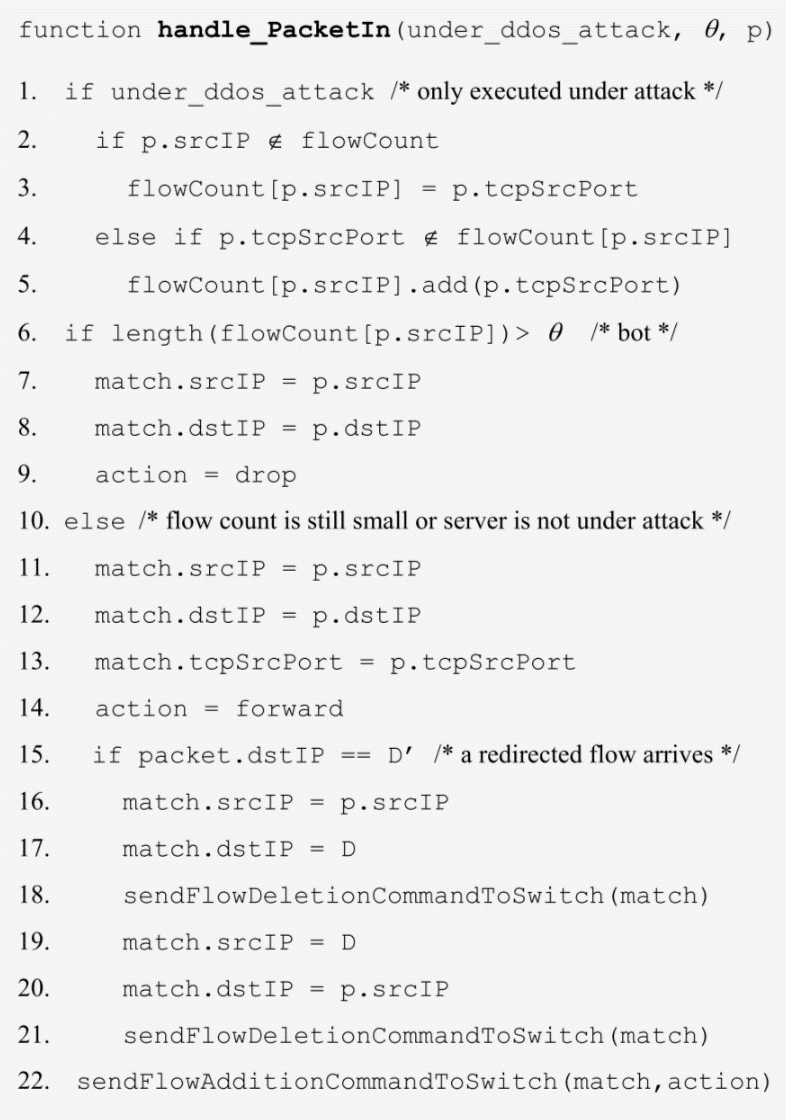
\includegraphics[width=\textwidth]{../images/PseudoCode.png}
\label{fig:pseudocode}
\caption{Pseudo code}
\end{center}
\end{figure}

We will implement a module inside ddosdefence-floodlight-controller/src/main/java/net/floodlightcontroller/ddosdefence here, there will be tree file: DDoSDefence.java, EnableDefenceResource.java IDDoSDefenceREST.java.